\documentclass[12pt]{article}
\usepackage{latexblog}

% ============================================================
% Blog Metadata
% ============================================================
\blogtitle{KDBX4 文件格式解析}
\blogdate{2019-03-07}
\blogtags{刨根问底, 协议}
\bloglang{zh}
\blogsummary{}

\begin{document}
\makeblogtitle

最近因为开始开发我自己的密码管理软件，因此对一些开源的密码管理软件做了一下研究，这其中一个比较著名的就是\href{https://keepass.info/}{KeePass}。KeePass将密码存在一个文本文件中，最新的格式是\href{https://keepass.info/help/kb/kdbx_4.html}{KDBX4}，官方的KeePass是在.Net平台上开发的，也有不少其他平台的移植版本，当然KDBX解析的库也比较多，可惜即便是官方文档也没有详细的描述。几经折腾找到了一个比较好的实现\href{https://keepassxc.org/}{Keepassxc}，这是一个基于c++和QT开发的跨平台版本，兼容Keepass的文件格式，我把代码做了精简就得到\href{https://github.com/soleverlee/keepass-client}{一个KDBX的操作库}，顺便调试了一下KDBX的文件格式，看看它是怎么存密码的。

\href{/images/ka.kdbx}{这里}有一个使用keepass创建的简单数据库，master密码是1125482715。

\begin{figure}
\centering
\pandocbounded{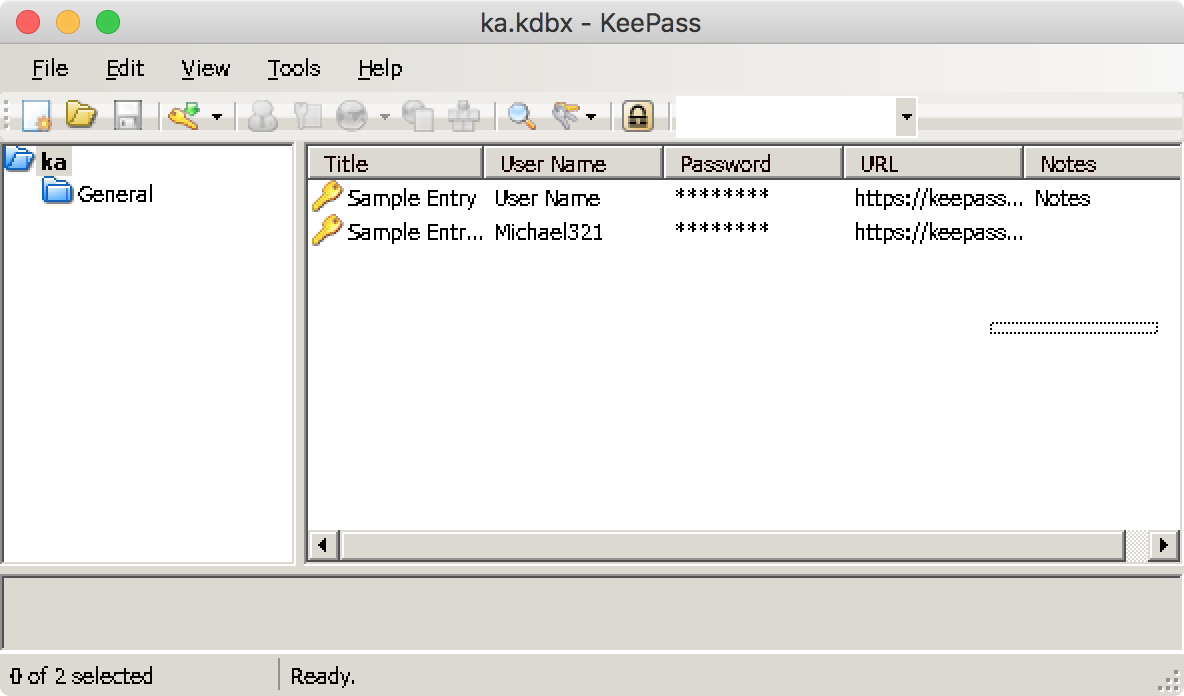
\includegraphics[keepaspectratio,alt={ka.kdbx}]{images/keepass_ka.png}}
\caption{ka.kdbx}
\end{figure}

\section{文件头（明文）}\label{ux6587ux4ef6ux5934ux660eux6587}

我们以十六进制形式打开文件可以看到这样的结构：

\begin{figure}
\centering
\pandocbounded{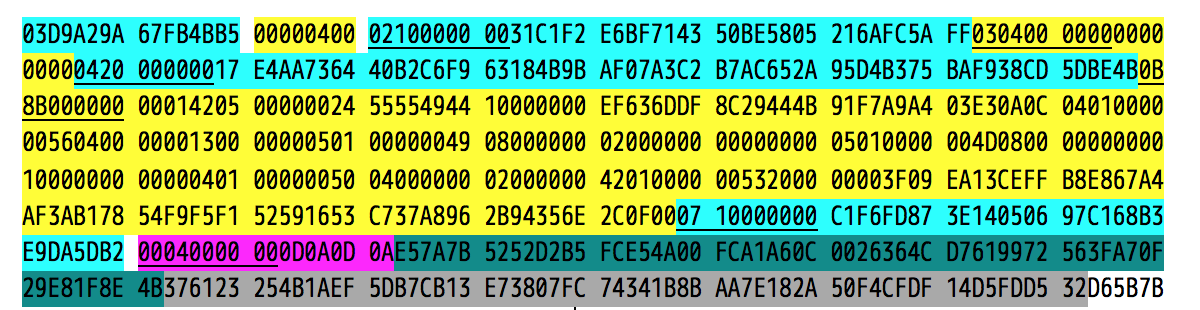
\includegraphics[keepaspectratio,alt={Hex of ka.kdbx}]{images/kdbx_hex_ka_header.png}}
\caption{Hex of ka.kdbx}
\end{figure}

\subsection{文件头格式}\label{ux6587ux4ef6ux5934ux683cux5f0f}

其中，文件头的结构可以用以下的形式来表述：

\[
Item_{i} = Id_{i} + Length + Data \\
Header = MagicNumber + Version + Item_{0} + ... + Item_{n} + Hash + Hmac
\]

首先，MagicNumber=\texttt{0x9AA2D903\ 0xB54BFB67}，代表这是KDBX文件格式

然后可以看到Version=\texttt{0x00040000}，目前有这样几种版本： - 0x00040000=4 - 0x00030001=3.1 - 0x00030000=3 - 0x00020000=2

然后是多个Header Item, 结构为{[}ID{]}{[}Length{]}{[}Data{]}，譬如\texttt{02100000\ 0031C1F2\ E6BF7143\ 50BE5805\ 216AFC5A\ FF}即代表id=0x02, length=0x00000010=16, data=0x31\textasciitilde0xFF。其中，这些ID中有一些特殊含义的ID：

\begin{verbatim}
EndOfHeader = 0,
Comment = 1,
CipherID = 2,
CompressionFlags = 3,
MasterSeed = 4,
TransformSeed = 5,
TransformRounds = 6,
EncryptionIV = 7,
ProtectedStreamKey = 8,
StreamStartBytes = 9,
InnerRandomStreamID = 10,
KdfParameters = 11,
PublicCustomData = 12
\end{verbatim}

所以这个Header就是表明加密算法，这些算法用UUID来标记：

\begin{itemize}
\tightlist
\item
  \texttt{0x31c1f2e6bf714350be5805216afc5aff} AES
\item
  \texttt{0xad68f29f576f4bb9a36ad47af965346c} TWOFISH
\item
  \texttt{0xD6038A2B8B6F4CB5A524339A31DBB59A} CHACHA20
\end{itemize}

\subsection{文件头校验}\label{ux6587ux4ef6ux5934ux6821ux9a8c}

在文件头的后面有两个比较特殊的段，存储了两个用来验证文件头正确性的字段：

\begin{itemize}
\tightlist
\item
  Header Hash(SHA-256)，即文件头的哈希值
\item
  Hmac(HMAC-SHA-256 )值，为文件头和密码一起加密后得出的值
\end{itemize}

通过计算哈希值能够判断文件头是否被人篡改，或者更准确的说是不是出现了损坏，因为如果真的被人篡改了，我相信他会连这个hash一起改掉，验证没有太大意义。因为KDB中数据采取了对称加密算法，而文件中也不会存储主密码，所以我们如何知道用户输入的密码是不是正确呢？

在Kdb以前的版本中，是尝试通过使用用户输入的密码去进行解密，如果出现问题或者解密出来的内容哈希值对不上，那么密码不对了。而在kdbx4中，采取了HMAC的方式，Hmac在哈希的基础上，加入了一个Key，意味着同一段数据，用不同的Key哈希之后的结果是不一样的。那么就可以根据用户输入的密码来计算Hmac值，如果和文件中记录的对不上，认为密码错误。

其实这个问题我也想过，我之前的想法是，把一段已知的明文加密后存储起来，然后再解密的时候，尝试用用户的密码加密后，来解密这个密文，看是否匹配。。当然如果这样做，需要考虑一下\href{https://zh.wikipedia.org/wiki/\%E5\%B7\%B2\%E7\%9F\%A5\%E6\%98\%8E\%E6\%96\%87\%E6\%94\%BB\%E5\%87\%BB}{已知明文攻击}。

\href{https://stackoverflow.com/questions/14493029/reliable-way-to-tell-if-wrong-key-is-used-in-aes256-decryption}{这里}还有有一个讨论可以参考。

\subsection{Key transform}\label{key-transform}

虽然不同的用户设置的密码都不一样，但通常我们在进行加密的时候，不会直接拿这个作为Key，而是会通过KDF \footnote{key derivation function} 将原始密码进行转换。keepass也不例外，我们这个文件设置的是使用Argon2来进行KDF，之前的版本采取的是AES-KDF。Keepass中转换的步骤如下:

\begin{enumerate}
\tightlist
\item
  将原始密码进行SHA-256转换，即 \[ sha256（1125482715）= d31d31dd2d99b5d35ce232896d0b3f1fe41daf6ba47b5c24d52e8890a0307da6 \]
\item
  再进行一次SHA-256 \[ sha256(d31d31dd2d99b5d35ce232896d0b3f1fe41daf6ba47b5c24d52e8890a0307da6) = \\ bfa11b4e4376cf1b17088a3de375f1df6a9c4cb3eb36f3ce2416b10481eb619f \]
\item
  将上次得到的哈希值，同header中配置的Transform seed进行KDF，得到最终的transformedMasterKey, 这里我们用的是argon2。\[ argon2d(2, 1024, pwd, salt) = \\
  104e9ba7b6b4479eec1a8fe3f9ca285fd10e0f33435fcabd8edf3e16380a98c7 \]这一步计算参见下面的代码：
\end{enumerate}

其中：\[ KdfSeed=3f09ea13ceffb8e867a4af3ab17854f9f5f152591653c737a8962b94356e2c0f \]

\begin{Shaded}
\begin{Highlighting}[]
\PreprocessorTok{\#include }\ImportTok{"argon2.h"}
\PreprocessorTok{\#include }\ImportTok{\textless{}stdio.h\textgreater{}}
\PreprocessorTok{\#include }\ImportTok{\textless{}stdlib.h\textgreater{}}

\DataTypeTok{int}\NormalTok{ main}\OperatorTok{(}\DataTypeTok{int}\NormalTok{ argc}\OperatorTok{,} \DataTypeTok{char}\OperatorTok{*}\NormalTok{argv}\OperatorTok{[])}
\OperatorTok{\{}
    \DataTypeTok{uint8\_t}\NormalTok{ pwd}\OperatorTok{[}\DecValTok{32}\OperatorTok{]} \OperatorTok{=} \OperatorTok{\{}\BaseNTok{0xbf}\OperatorTok{,} \BaseNTok{0xa1}\OperatorTok{,} \BaseNTok{0x1b}\OperatorTok{,} \BaseNTok{0x4e}\OperatorTok{,} \BaseNTok{0x43}\OperatorTok{,} \BaseNTok{0x76}\OperatorTok{,} \BaseNTok{0xcf}\OperatorTok{,} \BaseNTok{0x1b}\OperatorTok{,} \BaseNTok{0x17}\OperatorTok{,} \BaseNTok{0x08}\OperatorTok{,} \BaseNTok{0x8a}\OperatorTok{,} \BaseNTok{0x3d}\OperatorTok{,} \BaseNTok{0xe3}\OperatorTok{,} \BaseNTok{0x75}\OperatorTok{,} \BaseNTok{0xf1}\OperatorTok{,} \BaseNTok{0xdf}\OperatorTok{,} \BaseNTok{0x6a}\OperatorTok{,} \BaseNTok{0x9c}\OperatorTok{,} \BaseNTok{0x4c}\OperatorTok{,} \BaseNTok{0xb3}\OperatorTok{,} \BaseNTok{0xeb}\OperatorTok{,} \BaseNTok{0x36}\OperatorTok{,} \BaseNTok{0xf3}\OperatorTok{,} \BaseNTok{0xce}\OperatorTok{,} \BaseNTok{0x24}\OperatorTok{,} \BaseNTok{0x16}\OperatorTok{,} \BaseNTok{0xb1}\OperatorTok{,} \BaseNTok{0x04}\OperatorTok{,} \BaseNTok{0x81}\OperatorTok{,} \BaseNTok{0xeb}\OperatorTok{,} \BaseNTok{0x61}\OperatorTok{,} \BaseNTok{0x9f}\OperatorTok{\};}
    \DataTypeTok{uint8\_t}\NormalTok{ salt}\OperatorTok{[}\DecValTok{32}\OperatorTok{]} \OperatorTok{=} \OperatorTok{\{}\BaseNTok{0x3f}\OperatorTok{,} \BaseNTok{0x09}\OperatorTok{,} \BaseNTok{0xea}\OperatorTok{,} \BaseNTok{0x13}\OperatorTok{,} \BaseNTok{0xce}\OperatorTok{,} \BaseNTok{0xff}\OperatorTok{,} \BaseNTok{0xb8}\OperatorTok{,} \BaseNTok{0xe8}\OperatorTok{,} \BaseNTok{0x67}\OperatorTok{,} \BaseNTok{0xa4}\OperatorTok{,} \BaseNTok{0xaf}\OperatorTok{,} \BaseNTok{0x3a}\OperatorTok{,} \BaseNTok{0xb1}\OperatorTok{,} \BaseNTok{0x78}\OperatorTok{,} \BaseNTok{0x54}\OperatorTok{,} \BaseNTok{0xf9}\OperatorTok{,} \BaseNTok{0xf5}\OperatorTok{,} \BaseNTok{0xf1}\OperatorTok{,} \BaseNTok{0x52}\OperatorTok{,} \BaseNTok{0x59}\OperatorTok{,} \BaseNTok{0x16}\OperatorTok{,} \BaseNTok{0x53}\OperatorTok{,} \BaseNTok{0xc7}\OperatorTok{,} \BaseNTok{0x37}\OperatorTok{,} \BaseNTok{0xa8}\OperatorTok{,} \BaseNTok{0x96}\OperatorTok{,} \BaseNTok{0x2b}\OperatorTok{,} \BaseNTok{0x94}\OperatorTok{,} \BaseNTok{0x35}\OperatorTok{,} \BaseNTok{0x6e}\OperatorTok{,} \BaseNTok{0x2c}\OperatorTok{,} \BaseNTok{0x0f}\OperatorTok{\};}
    \DataTypeTok{uint8\_t}\NormalTok{ result}\OperatorTok{[}\DecValTok{32}\OperatorTok{];}
    \CommentTok{// argon2: seed=kef.seed, version=19, rounds=2, memory=1024, parallelism=2}
\NormalTok{    argon2\_hash}\OperatorTok{(}\DecValTok{2}\OperatorTok{,} \DecValTok{1024}\OperatorTok{,} \DecValTok{2}\OperatorTok{,}\NormalTok{ pwd}\OperatorTok{,} \DecValTok{32}\OperatorTok{,}\NormalTok{ salt}\OperatorTok{,} \DecValTok{32}\OperatorTok{,}\NormalTok{ result}\OperatorTok{,} \DecValTok{32}\OperatorTok{,} \KeywordTok{nullptr}\OperatorTok{,} \DecValTok{0}\OperatorTok{,}\NormalTok{ Argon2\_d}\OperatorTok{,} \DecValTok{19}\OperatorTok{);}
    \ControlFlowTok{for}\OperatorTok{(}\DataTypeTok{int}\NormalTok{ i }\OperatorTok{=} \DecValTok{0}\OperatorTok{;}\NormalTok{ i }\OperatorTok{\textless{}} \DecValTok{32}\OperatorTok{;}\NormalTok{ i }\OperatorTok{++)}
\NormalTok{        printf}\OperatorTok{(}\StringTok{"}\SpecialCharTok{\%02x}\StringTok{"}\OperatorTok{,}\NormalTok{ result}\OperatorTok{[}\NormalTok{i}\OperatorTok{]);}
\OperatorTok{\}}
\end{Highlighting}
\end{Shaded}

\subsection{Hmac计算}\label{hmacux8ba1ux7b97}

另一个就是HMac值的计算了，首先需要算出一个Key，在keepass中是这样去算的:

\[
Key1 = sha512(MasterSeed + TransformedMasterKey + 0x01)
\]

\begin{verbatim}
sha512(17e4aa736440b2c6f963184b9baf07a3c2b7ac652a95d4b375baf938cd5dbe4b104e9ba7b6b4479eec1a8fe3f9ca285fd10e0f33435fcabd8edf3e16380a98c701)
= 9340685dcea0fbee49a68417708cbffb24958fc6fb20de6cb158196b6291f0719f46669bbc8f7254bcbc0da0650d795fe9c782e443d3f32b7a957f73c8f58128
\end{verbatim}

然后需要把这个key再计算一下:

\[
Key = sha512(BlockIndex + Key1)
\]

\begin{verbatim}
sha512(ffffffffffffffff9340685dcea0fbee49a68417708cbffb24958fc6fb20de6cb158196b6291f0719f46669bbc8f7254bcbc0da0650d795fe9c782e443d3f32b7a957f73c8f58128)
=1062ee78cf505ac4af4e53f343b04782178a3c6d6b8e64ecb23ca6ce9489ab30660b92cf1f88dbf0333769e9f362ae2d7dff82554d864a4c2d1d3b751b5698f7
\end{verbatim}

这个Key才是最终用来计算Hmac的Key:

\[
HmacValue = Hmac-sha256(header, Key)
\]

\begin{verbatim}
Hmac-sha256(03D9A29A67FB4BB500000400021000000031C1F2E6BF714350BE5805216AFC5AFF030400000000000000042000000017E4AA736440B2C6F963184B9BAF07A3C2B7AC652A95D4B375BAF938CD5DBE4B0B8B00000000014205000000245555494410000000EF636DDF8C29444B91F7A9A403E30A0C040100000056040000001300000005010000004908000000020000000000000005010000004D0800000000001000000000000401000000500400000002000000420100000053200000003F09EA13CEFFB8E867A4AF3AB17854F9F5F152591653C737A8962B94356E2C0F000710000000C1F6FD873E14050697C168B3E9DA5DB200040000000D0A0D0A, 1062ee78cf505ac4af4e53f343b04782178a3c6d6b8e64ecb23ca6ce9489ab30660b92cf1f88dbf0333769e9f362ae2d7dff82554d864a4c2d1d3b751b5698f7)
=376123254b1aef5db7cb13e73807fc74341b8baa7e182a50f4cfdf14d5fdd532
\end{verbatim}

\section{文件内容（Encrypted)}\label{ux6587ux4ef6ux5185ux5bb9encrypted}

\subsection{秘钥计算}\label{ux79d8ux94a5ux8ba1ux7b97}

在文件头后面，跟着的是文件的数据内容了，这部分数据是加密过的。因此首先需要知道是根据什么样的秘钥进行加密的。其实很简单:

\[
Key = sha256 (MasterSeed + TransformedMasterKey)
\]

\begin{verbatim}
sha256(17E4AA736440B2C6F963184B9BAF07A3C2B7AC652A95D4B375BAF938CD5DBE4B104e9ba7b6b4479eec1a8fe3f9ca285fd10e0f33435fcabd8edf3e16380a98c7)
=dce60234d641f71f377ecafb5a566ce954d26c03fd3b5b23e9ed092ef42b5290
\end{verbatim}

所以这个文件中，解密是这样的：

\begin{verbatim}
Key=dce60234d641f71f377ecafb5a566ce954d26c03fd3b5b23e9ed092ef42b5290
Iv=c1f6fd873e14050697c168b3e9da5db2

9a0106470245744f9121bbafa5dd10df => 01040000000300000002400000008B2E
\end{verbatim}

这里需要指出的是，这里应该使用AES-CBC-NoPadding算法，这样加密后的密文和原文是一样的长度，否则会变长。而且解密的时候，是一段一段的解的，16byte一截。

\begin{Shaded}
\begin{Highlighting}[]
\KeywordTok{public} \DataTypeTok{static} \DataTypeTok{byte}\OperatorTok{[]} \FunctionTok{decrypt}\OperatorTok{(}\DataTypeTok{byte}\OperatorTok{[]}\NormalTok{ key}\OperatorTok{,} \DataTypeTok{byte}\OperatorTok{[]}\NormalTok{ initVector}\OperatorTok{,} \DataTypeTok{byte}\OperatorTok{[]}\NormalTok{ encrypted}\OperatorTok{)} \OperatorTok{\{}
        \ControlFlowTok{try} \OperatorTok{\{}
            \BuiltInTok{IvParameterSpec}\NormalTok{ iv }\OperatorTok{=} \KeywordTok{new} \BuiltInTok{IvParameterSpec}\OperatorTok{(}\NormalTok{initVector}\OperatorTok{);}
            \BuiltInTok{SecretKeySpec}\NormalTok{ skeySpec }\OperatorTok{=} \KeywordTok{new} \BuiltInTok{SecretKeySpec}\OperatorTok{(}\NormalTok{key}\OperatorTok{,} \StringTok{"AES"}\OperatorTok{);}

            \BuiltInTok{Cipher}\NormalTok{ cipher }\OperatorTok{=} \BuiltInTok{Cipher}\OperatorTok{.}\FunctionTok{getInstance}\OperatorTok{(}\StringTok{"AES/CBC/NoPadding"}\OperatorTok{);}
\NormalTok{            cipher}\OperatorTok{.}\FunctionTok{init}\OperatorTok{(}\BuiltInTok{Cipher}\OperatorTok{.}\FunctionTok{DECRYPT\_MODE}\OperatorTok{,}\NormalTok{ skeySpec}\OperatorTok{,}\NormalTok{ iv}\OperatorTok{);}

            \ControlFlowTok{return}\NormalTok{ cipher}\OperatorTok{.}\FunctionTok{doFinal}\OperatorTok{(}\NormalTok{encrypted}\OperatorTok{);}
        \OperatorTok{\}} \ControlFlowTok{catch} \OperatorTok{(}\BuiltInTok{Exception}\NormalTok{ ex}\OperatorTok{)} \OperatorTok{\{}
\NormalTok{            ex}\OperatorTok{.}\FunctionTok{printStackTrace}\OperatorTok{();}
        \OperatorTok{\}}

        \ControlFlowTok{return} \KeywordTok{null}\OperatorTok{;}
    \OperatorTok{\}}
\end{Highlighting}
\end{Shaded}

\subsection{Inner Header}\label{inner-header}

Inner Header跟Header结构一样，对应了如下的类型：

\begin{verbatim}
0x00: End of header.
0x01: Inner random stream ID (this supersedes the inner random stream ID stored in the outer header of a KDBX 3.1 file).
0x02: Inner random stream key (this supersedes the inner random stream key stored in the outer header of a KDBX 3.1 file).
0x03: Binary (entry attachment). D = F ‖ M, where F is one byte and M is the binary content (i.e. the actual entry attachment data). F stores flags for the binary; supported flags are:
    0x01: The user has turned on process memory protection for this binary.
\end{verbatim}

\subsection{XML Database}\label{xml-database}

Inner Header之后一大段就是XML加密后的内容了，直接解密就可以了。解密出来其实就是个XML。这里就不过多解释了。 最终结构就是如图所示了：

\pandocbounded{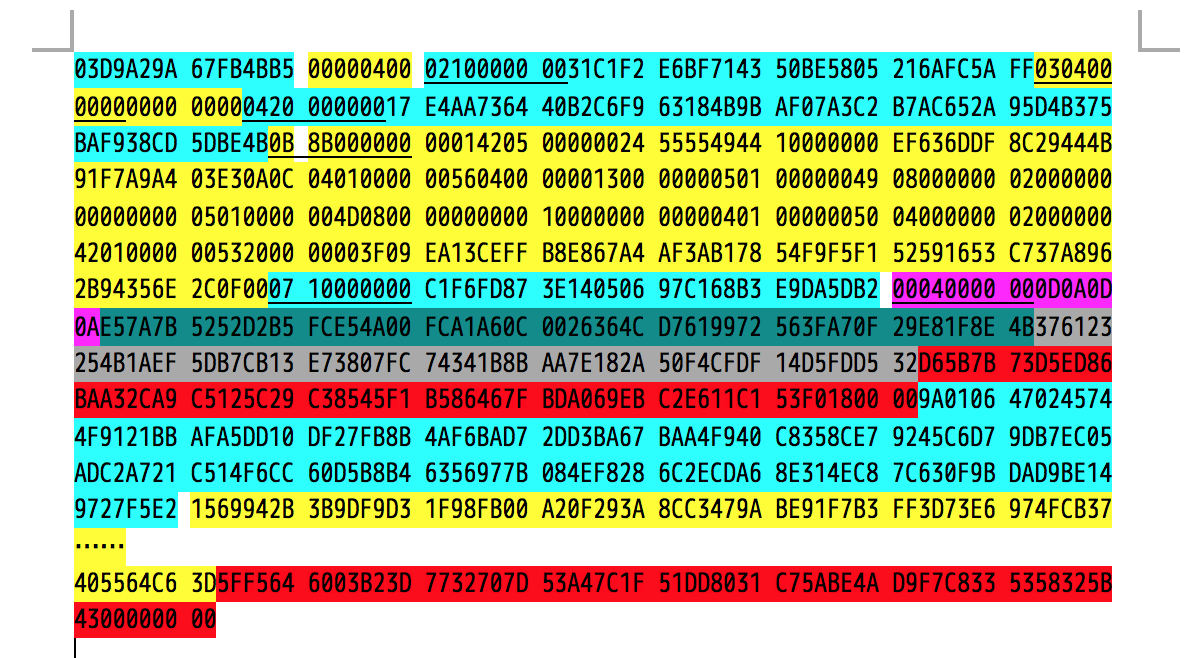
\includegraphics[keepaspectratio,alt={Hex of ka.kdbx}]{images/keepass_hex_sturcture.png}}，

目前还有两个地方没大搞懂的就是，标红的地方，就是加密的部分开头和结尾的，不知道有何用，代码嵌套的挺深的，看了下没找到地方，各个文档中也没说清楚，不过可以肯定的是，这两个地方用到了。有时间再看吧。

References:

\begin{itemize}
\tightlist
\item
  \href{https://cryptii.com/pipes/aes-encryption}{Cryptii}
\item
  \href{https://www.devglan.com/online-tools/aes-encryption-decryption}{AES Encryption and Decryption Online Tool(Calculator)}
\item
  \href{http://extranet.cryptomathic.com/hashcalc/index}{Hash}
\item
  \href{https://github.com/Evidlo/keepassxc-specs/blob/master/kdbx-binary/kdbx4_overview.md}{overview for KDBX4}
\item
  \href{https://gist.github.com/msmuenchen/9318327}{KeePass v2.x (KDBX v3.x) file format}
\item
  \href{https://gist.github.com/lgg/e6ccc6e212d18dd2ecd8a8c116fb1e45}{Keepass file format explained}
\end{itemize}


\end{document}
